% В этом шаблоне используется класс spbau-diploma. Его можно найти и, если требуется, 
% поправить в файле spbau-diploma.cls
\documentclass{spbau-diploma}
\usepackage{pdfpages}
\usepackage{subfiles}
\usepackage{listings}
\usepackage{xcolor}
\usepackage{minted}
\usepackage{caption}
\usepackage{hyperref}
\usepackage[noend]{algpseudocode}
\usepackage{algorithm}
\usepackage{amssymb}
\usepackage[stable]{footmisc}
\begin{document}
\renewcommand\listingscaption{Листинг}
\newenvironment{megaalgorithm}[1][htb]{
    \floatname{algorithm}{Алгоритм}%% Update algorithm name
   \begin{algorithm}%
  }{\end{algorithm}}

% Год, город, название университета и факультета предопределены,
% но можно и поменять.
% Если англоязычная титульная страница не нужна, то ее можно просто удалить.
\filltitle{ru}{
    title              = {Переоснащение неявных модулей для языка 1ML},
    type               = {bachelor},
    position           = {студента},
    group              = БПМ171,
    author             = {Трилис Алексей Андреевич},
    supervisorPosition = {к.\,ф.-м.\,н.},
    supervisor         = {Березун Д.\,А.},
}
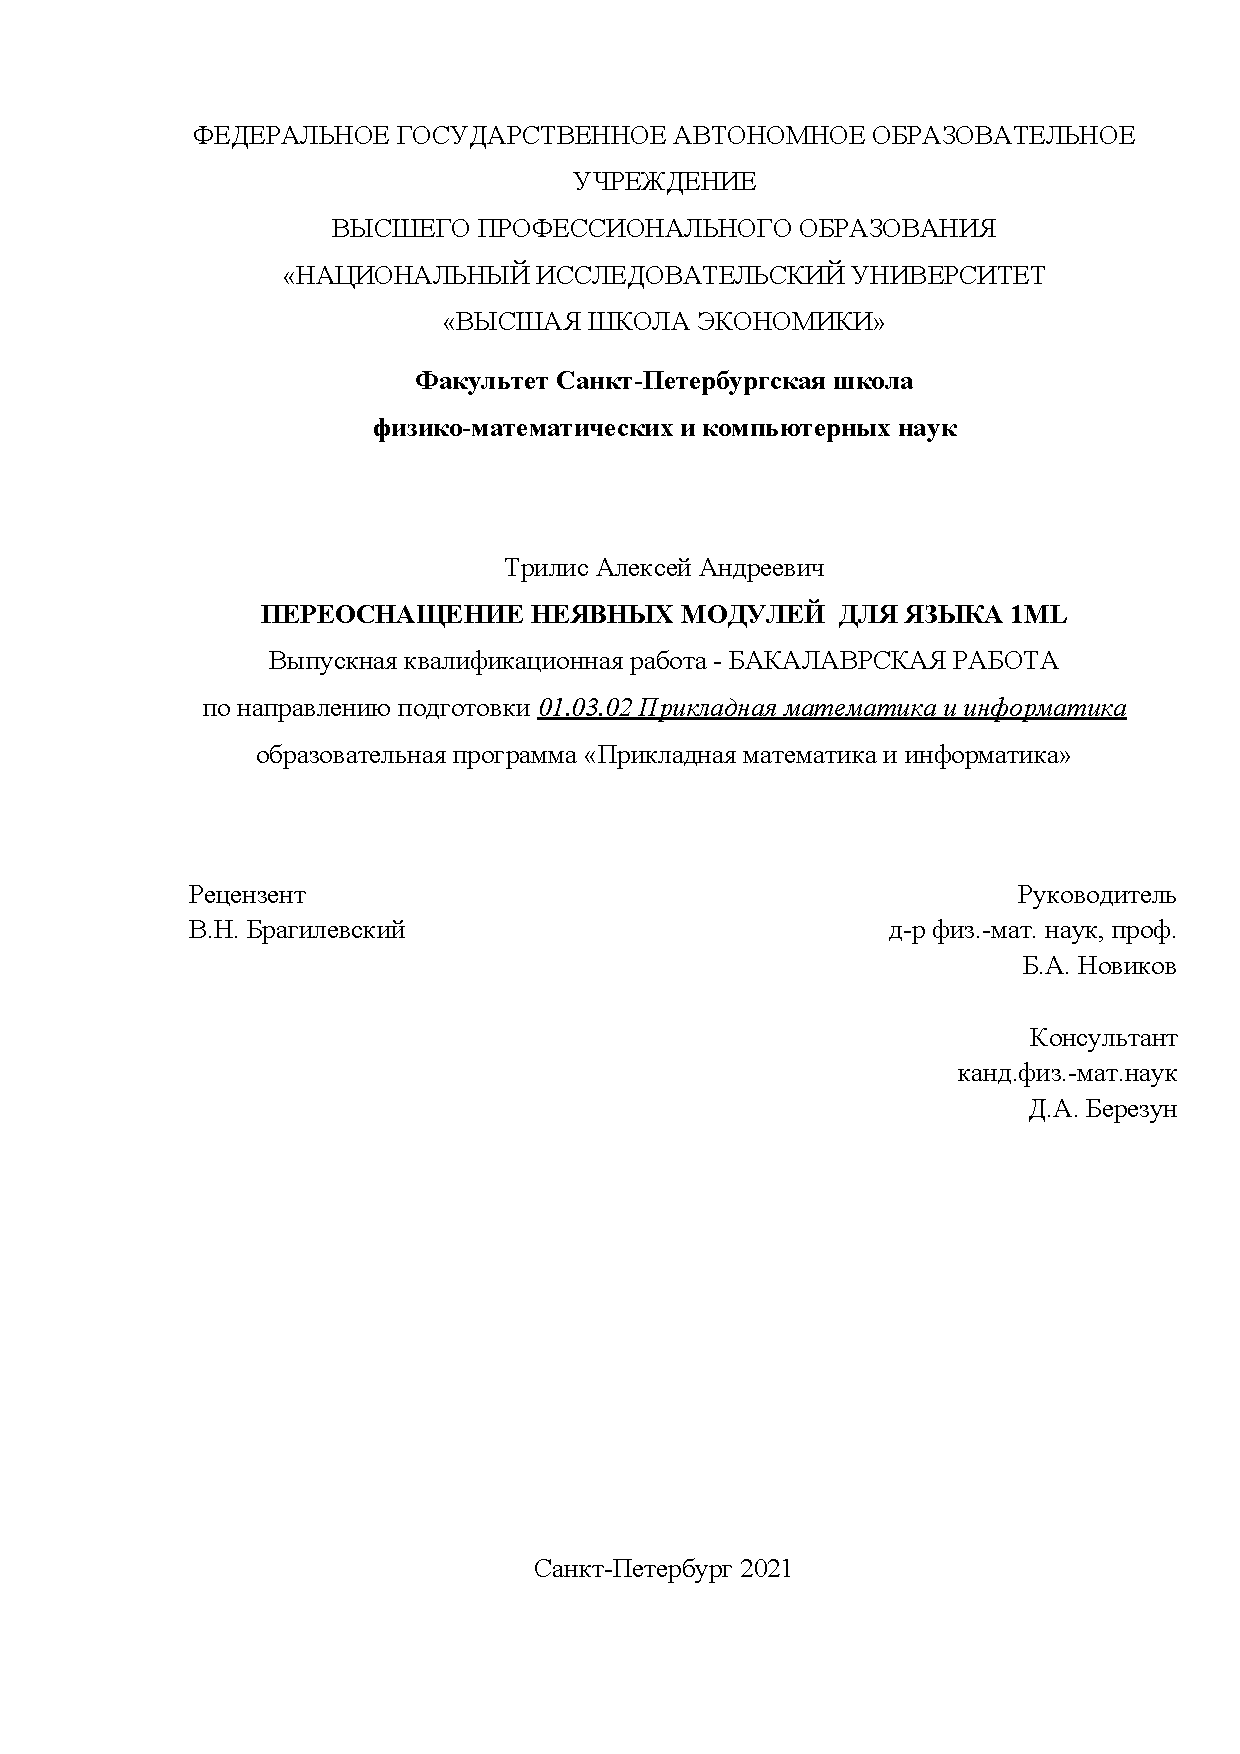
\includepdf[pages=-]{title.pdf}
\maketitle
\setcounter{page}{2}
\tableofcontents


\section*{Аннотация}
\subfile{sections/abstract}

\section*{Введение}
\subfile{sections/introduction}

\section{Обзор литературы}
\subfile{sections/domain_review}

\section{Синтаксис, семантика, описание алгоритма}
\subfile{sections/1}

\section{Детали решения и примеры использования}
\subfile{sections/2}

\section{Порядок разрешения}
\subfile{sections/3}

\section*{Заключение}
\subfile{sections/conclusion}


\bibliographystyle{ugost2008my}
\bibliography{diploma.bib}
\end{document}
